\documentclass{article}
\usepackage{import}
\subimport{../}{preamble}
\begin{document}

\section{Modified Method for Controllable Fabrication of Spherical AuNP Tips}

\begin{figure}[bt]
\centering
\fontsize{10pt}{1em}\selectfont
\subimport{./figures/}{new_setup.pdf_tex}
\caption[Diagram of the modified method for electrochemical AuNP tip fabrication.]{\textbf{Diagram of the modified electrochemical cell for electrochemical AuNP tip fabrication.} The ITO glass active electrode used for simultaneous fabrications is removed and replaced with an aluminium clamp fitting a single tip along with the addition of a Pt reference electrode. Over potentials are now measured relative to the reference electrode.}
\label{fig:new_method}
\end{figure}

% The new method
The previous method of fabrication provided a means of demonstrating that electrodeposition can be used to produce spherical tip apices but failed to give sufficient reliability or understanding of growth due to the variability in the FTO working electrode contact resistance and scale with respect to the attached tips. A modified cell geometry for pulsed electrodeposition on a single tip improves upon the fabrication process. The setup, shown in \figurename~\ref{fig:new_method}, does not have the capability of simultaneously depositing on multiple tips but provides more control and monitoring of the growth of a single tip.

% Why use Pt and not Au - is it plasmonic/dielectric?
To retain good plasmonic confinement to the spherical AuNP apex, Pt-coated AFM tips are used as a base structure to maintain an electromagnetic boundary between the AuNP and the tip.
% Pre-treatments
A \SI{10}{\minute} \ce{O2} plasma pretreatment is still used to clean tips before electrodeposition.
% Addition of Pt reference electrode
A compact potentiostat (Ivium CompactStat) replaces the larger potentiostat and a 3d-printed electrode support frame is used for stability.%
\footnote{3d-printed support frame designed and printed by Richard W. Bowman.}
Controllability is improved by measuring the current during electrodeposition more carefully and referencing the potential using a Pt wire electrode. As stated previously, Pt wire is chosen as a reference electrode as its high conductivity maintains a high measurement bandwidth during 10--\SI{100}{ms} time scale pulsed deposition \cite{sawyer1995electrochemistry}.
% Change of active electrode
The quality of the tip contact with the working electrode is a large factor limiting the reproducibility between repeated experiments in the initial method. Unreliable contacting of the tips to the FTO glass is likely to be the dominant cause. This is improved in the new method by replacing the FTO glass with an aluminium clamp capable of holding a single tip. Though it prevents simultaneous fabrication of multiple tips, the clamp provides a reliable, highly conductive contact. The potential at the apex is therefore held stably at the applied potential.

% Major changes
The major consequence of the changes made to the setup is that the required applied over-potential is different. The previously valid voltages of $-6$ to \SI{-8}{V} no longer produce successful growths and the system requires optimising with new parameters. Since the working electrode potential is now relative to the solution, rather than the counter electrode, the magnitude of the overpotential decreases. The result of this is that successful fabrications occur mostly around \SI{-3}{V}. This is more comparable to reported nucleation over-potentials, as measured relative to a \gls{she}, more negative than \SI{-1}{V} \cite{}. Similar exposure times are still used.

\begin{figure}[bt]
\centering
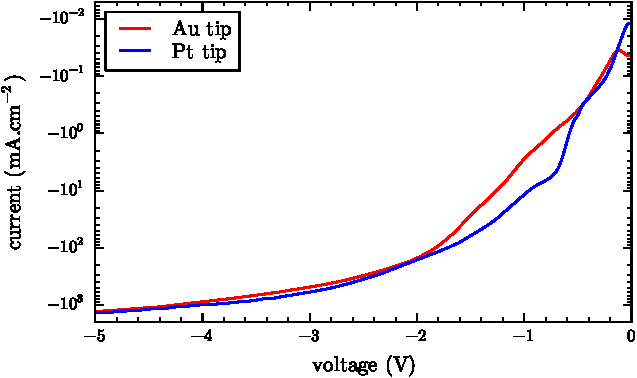
\includegraphics{figures/linear_sweep_measurements}
\caption[]{Linear sweep measurements}
\label{fig:linear_sweeps}
\end{figure}

Linear voltage sweep measurements of both Au and Pt tips (\figurename~\ref{fig:linear_sweeps}) show that the onset of growth is earlier for Pt. Pt's use as a catalyst may be the cause of this reduction in reaction energy.

% Changes to solution
\begin{figure}[h]
\centering
\begin{subfigure}[t]{0.48\textwidth}
\caption[Diffusion-limited currents during electrodeposition for different potentials.]{\textbf{Diffusion-limited currents during electrodeposition for different potentials.}}
\label{fig:voltage_saturation_current}
\end{subfigure}
\ \
\begin{subfigure}[t]{0.48\textwidth}
\caption[Comparison of growth localisation at different potentials.]{\textbf{Comparison of growth localisation at different potentials.} The more negative the potential the more localised growth is to the apex.}
\label{fig:growth_localisation}
\end{subfigure}
\caption{Both growth localisation and current increase with more negative potentials.}
\end{figure}

The more negative the potential the more localised growth is to the apex (\figurename~\ref{fig:growth_localisation}). However with large overpotentials comes a large current and therefore a need to decrease exposure. For every \SI{-1}{V} added to the potential () the current approximately  increases by a factor of 10 (\figurename~\ref{fig:voltage_saturation_current}). To control deposition more effectively the current is reduced by diluting the {\color{red}ECF60/electrolyte}. This allows nucleation to occur during electromigration-limited growth on short time-scales before the restricted diffusion flow cuts it off causing only growth to pre-existing nuclei. Diluting by 50\% reduces the current by approximately a factor of 10, hence more localised growth at \SI{-4}{V} becomes more controllable using exposure times previously used at \SI{-3}{V}.

% Pre-processing
%\begin{figure}[bt]
%\centering
%\caption[Comparison of pre-treatments on growth morphology.]{\textbf{Comparison of pre-treatments on growth morphology.}}
%\label{fig:pre_treatment_comparison}
%\end{figure}

%The effects of pre-treatments on growth morphology are investigated by comparing different length \ce{O2} plasma treatments and treatment with piranha solution (3:1 \ce{H2SO4}:\ce{H2O2}). Both plasma treatment and piranha solution are confirmed to remove {\color{red}organic(s) molecules/residue} from Au surfaces \cite{}, and both are able to oxidise the surface \cite{}, however plasma is the more extreme treatment.

%Typical pre-treatment of Pt AFM probes prior to electrodeposition is \SI{20}{\minute} \ce{O2} plasma to oxidise the surface. This protects the flat surfaces from growth aiding localisation of Au to the tip apex. Plasma treatment less than 20 minutes results in insufficient protection allowing growth across the whole surface while exposures longer than 30 minutes result in what appears to be severe damage to the AFM probe. This is potentially full oxidation of the Pt coating and oxidation of the Si to expanded \ce{SiO2} beneath the surface, which gives the surface its rough appearance in SEM. Piranha pre-treatment (\SI{1}{\hour}, \SI{7}{ml} volume) should also oxidise surfaces but showed no observable difference to untreated tips after deposition. The extreme conditions of plasma treatment are therefore seemingly required for successful surface preparation.

% Post-processing
Imaging tips using SEM after electrodeposition is necessary to determine the apex morphology but leads to contamination issues. Exposure to the electron beam is known to deposit layers of carbon onto samples. Despite washing tips in DI water and ethanol after deposition to remove thin films, the surface of the tip inevitably has carbon contamination after imaging. To ensure good electrical contact, AuNP-on-Pt tips must be cleaned before use. Although plasma cleaning is used to remove organics from the surface before fabrication it can oxidise the surface. Submerging tips in piranha solution (3:1 \ce{H2SO4}:\ce{H2O2}) proves to be an effective method for removing organics from the surface of the Au. Though it can still oxidise {\color{red}(or hydroxylate)} surfaces it is to a lesser extent compared to plasma treatment since it is much less extreme.%
% How piranha works
\footnote{Piranha solution is a strong oxidising agent and works via \ce{H2SO4} quickly dehydrating the surface. The reaction between \ce{H2SO4} and \ce{H2O2} creates oxygen radicals which oxidise the remaining carbon molecules into elemental carbon. The overall result is the decomposition of organic matter into carbon, carbon dioxide and water.} The activity of piranha solution degrades over time and the solution is only effective for $\sim$\SI{15}{\minute}. During its initial stages, the piranha reaction is extremely exothermic with temperatures reaching up to \SI{120}{\celsius}. The amount of heat generated is limited by the volume of solution used.

\begin{figure}[bt]
\centering
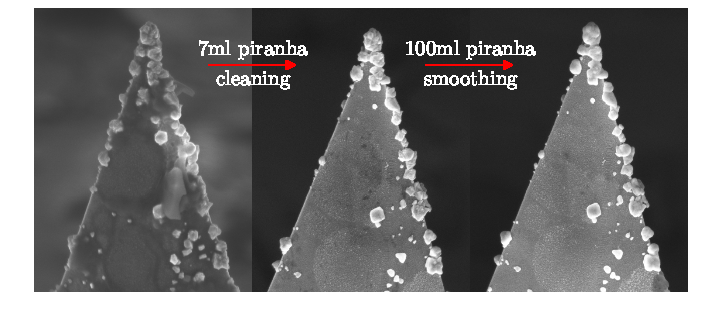
\includegraphics[clip=true, trim=20 20 0 0]{figures/tip_post_processing}
\caption[Post-processing effects of piranha solution.]{\textbf{Post-processing effects of piranha solution.} Low volume and temperature piranha solution removes organics from the Au surface while large volumes at \SI{120}{\celsius} smooth the surface.}
\label{fig:tip_post_processing}
%\vspace{-5pt}
\end{figure}

% Temperature effects
Tips treated with piranha solution contacted {\color{red}significantly more often than} tips left untreated after SEM imaging. The morphology of tips can be somewhat adjusted by varying the temperature and exposure to the piranha solution. Piranha treatment is a heavily exothermic reaction with temperatures reaching up to \SI{120}{\celsius}. The temperature depends on the volume of solution. Tips cleaned in small (\SI{5}{ml}) volumes show no changes in morphology whereas those treated in a large (\SI{100}{ml}) volumes are found to have their surfaces smoothed (\figurename~\ref{fig:tip_post_processing}).
% The effects of this on the plasmonic nanofocussing are as yet undetermined. Also comparison with furnace.

Gold etching solution (Sigma) is used to remove deposited Au from Pt tips, returning them back to their original condition. This means failed fabrications can be reset and attempted again, reducing the effective cost per successfully nanostructured tip.

\end{document}